\chapter{Divide et impera}
\begin{redbar}
Un programma sviluppato secondo questa tecnica è sostanzialmente diviso in tre parti:
\begin{itemize}
    \item \textit{Divide:} in questa parte si procede alla suddivisione dei problemi in problemi di dimensione minore;
    \item \textit{Impera:} nella seconda parte i problemi vengono risolti in modo ricorsivo. Quando i sottoproblemi arrivano ad avere una dimensione sufficientemente piccola, essi vengono risolti direttamente tramite il caso base; 
    \item \textit{Combina:} l'ultima fase del paradigma prevede di ricombinare l'output ottenuto dalle precedenti chiamate ricorsive al fine di ottenere il risultato finale.
\end{itemize}
\end{redbar}

Quali sono i vantaggi offerti da questa tecnica? Di solito, quando la tecnica è applicabile, non è difficile vedere come applicarla. Questo perché, tipicamente, è facile intuire come si potrebbe spezzare l'istanza. Inoltre, è abbastanza facile, una volta che un algoritmo di Divide et Impera è stato ideato, analizzarne sia la correttezza che la complessità. In particolare, la complessità di un algoritmo Divide et Impera, essendo un algoritmo ricorsivo, può essere determinata risolvendo un'opportuna relazione di ricorrenza relativa alla funzione $T(n)$ che dà il massimo tempo di calcolo dell'algoritmo su istanze di dimensione $n$.

\section{Algoritmi divide et impera}
\subsection{Problema della selezione}
\textit{Data una lista $A$ di interi distinti, il rango di un elemento in $A$ è il numero di elementi che sono minori o uguali ad $x$ in $A$. Ad esempio il minimo in $A$ è l'elemento di rango 1, il mediano in $A$ è l'elemento di rango $\frac{n}{2}$ e il massimo in $A$ è l'elemento di rango $n$.
Abbiamo una lista $A$ di $n$ numeri distinti ed un intero $k$, $1\leq k \leq n$. Vogliamo l'elemento di rango $k$ in $A$.}

Un semplice algoritmo di complessità $O(n\log n)$ è il seguente:
\begin{lstlisting}[language=Python]
    def selezionel(A, k):
        A.sort()
        return A[k-1]
\end{lstlisting}

Se $k=1$ o $k=n$ il problema si riduce alla ricerca del minimo o del massimo e questi casi sono risolvibili in tempo $\Theta(n)$.
Utilizzando la tecnica del divide et impera, vedremo che, anche nel caso generale, il problema può risolversi in $\Theta(n)$. In altre parole dimostreremo che il problema della selezione è computazionalmente più semplice di quello dell'ordinamento (che richiede tempo $\Omega(n\log n)$).

\subsubsection{Approccio basato sul divide et impera}
L'approccio basato sul divide et impera segue questi passi:
\begin{enumerate}
    \item scegli nella lista $A$ un elemento $x$ (che chiameremo perno);
    \item a partire da $A$ costruisci due liste $A_1$ ed $A_2$, la prima contenente gli elementi di $A$ minori di $x$ e la seconda gli elementi di $A$ maggiori di $x$.
    \item dove si trova l'elemento di rango $k$? Se $|A_1| \geq k$ allora l'elemento di rango $k$ è nel vettore $A_1$; se $|A_1| = k - 1$ allora l'elemento di rango $k$ è proprio il perno $x$; se $|A_1| < k - 1$ allora l'elemento di rango $k$ è in $A_2$ è l'elemento di rango $k - |A_1| - 1$ in $A_2$.
\end{enumerate}
Nota che dopo aver costruito dalla lista $A$ di elementi le due liste $A_1$ e $A_2$, grazie al test sulla cardinalità di $A_1$ il problema della selezione dell'elemento di rango $k$ o risulta risolto o viene ricondotto alla selezione di un elemento in una lista con meno di $n$ elementi.

\begin{lstlisting}[language=Python]
    def selezione2(A, k):
        if len(A)==1:
            return A[0]
        perno=A[0]
        A1, A2= [], []
        for x in A:
            if x < perno:
                A1.append(x)
            elif x > perno:
                A2.append(x)
        if len(A1) >= k:
            return selezione2(A1, k)
        elif len(A1) == k-1:
            return perno
        return selezione2(A2, k-len(A1)-1)
\end{lstlisting}
La procedura che tripartisce la lista in $A_1$, $p$ e $A_2$ può restituire una partizione massimamente sbilanciata in cui si ha ad esempio $|A_1|=0$ e $|A_2|=n-1$, questo accade quando il perno $p$ risulta l'elemento minimo nella lista.

Qualora questo evento sfortunato si ripetesse sistematicamente nel corso delle varie partizioni eseguite dall'algoritmo (questo può accadere quando cerco il massimo in una lista ordinata), allora la complessità dell'algoritmo al caso pessimo viene catturata dalla seguente equazione:
\begin{equation*}
    T(n)=T(n-1)+ \Theta(n)    
\end{equation*}
che risolta dà
\begin{equation*}
    T(n) = \Theta(n^2)    
\end{equation*}
In generale la complessità superiore alla procedura è catturata dalla ricorrenza
\begin{equation*}
    T(n) = T(m) + \Theta(n)    
\end{equation*}
dove $m = max\{|A_1|,|A_2|\}$.

Se avessimo una regola di scelta del perno $p$ in grado di garantire una partizione perfettamente bilanciata (vale a dire $m=max(\{|A_1|, |A_2|\}\approx n/2$) allora per la complessità $T(n)$ dell'algoritmo avremmo
\begin{equation*}
    T(n) = T\left(\frac{n}{2}\right) + \Theta(n)
\end{equation*}
che produce $T(n) = \Theta(n)$.

Chiedere che la partizione sia perfettamente bilanciata è forse chiedere troppo, potremmo allora accontentarci di chiedere che la scelta del perno $p$ garantisca partizioni non troppo sbilanciate come ad esempio quelle per cui $m\approx 3n/4$. In questo caso si ha
\begin{equation*}
    T(n) )\leq T\left(\frac{3}{4}n\right)+\Theta(n)
\end{equation*}
che risolta dà ancora $T(n) = \Theta(n)$.
In generale finché $m$ è una frazione di $n$ (anche piuttosto vicina ad $n$ come ad esempio $\frac{99}{100}n$) la ricorrenza da sempre $T(n) = \Theta(n)$.

Scegliamo il perno $p$ a caso in modo equiprobabile tra gli elementi della lista.
Anche se la scelta "casuale" non produce necessariamente una partizione bilanciata, quanto visto ci fa intuire che la complessità rimane lineare in $n$.

\begin{lstlisting}[language=Python]
    from random import randint

    def selezione2R(A, k)
        if len(A)==1:
            return A[0]
        perno=A[randint(0, len(A)-1)]
        A1, A2 = [], []
        for x in A:
            if x < perno:
                A1.append(x)
            elif x > perno:
                A2.append(x)
        if len(A1)>=k:
            return selezione2R(A1, k)
        elif len(A1)==k-1:
            return perno
        return selezione2R(A2, k-len(A1)-1)
\end{lstlisting}

\subsubsection{Analisi formale del caso medio}
Più formalmente, sotto l'assunzione che il pivot possa essere con uguale probabilità un elemento di qualsiasi rango tra 1 e $n$ la ricorrenza la ricorrenza da studiare per il caso medio è
\begin{equation*}
    T(n) \leq \frac{1}{n}\sum_{k=1}^n T(max(T(k-1), T(n-k))) + \Theta(n) = \frac{1}{n}\sum_{k=1}^{n-1}2T(k) + \Theta(n) \textit{ per } n\geq 2
\end{equation*}
possiamo dimostrare che per questa ricorrenza vale $T(n)=O(n)$ col metodo di sostituzione.
Sia $T(n)\leq \frac{1}{n}\sum_{k=\frac{n}{2}}^{n-1}2T(k)+a*n \textit{ per } n \geq 3$, $T(x) \leq b$ altrimenti e dimostriamo $T(n) \leq cn$ per una $c > 0$ costante.
Per $n \leq 3$ abbiamo $T(n) \leq b \leq 3c$ che vera ad esempio per $c \geq b$.
Per ipotesi induttiva abbiamo $T(n)\leq \frac{2c}{n}\sum_{k=\frac{n}{2}}^{n-1}k+a*n$ da cui ricaviamo

\begin{align*}
    T(n)\leq \frac{2c}{n}\left(\sum^{n-1}_{k=1}k-\sum^{\frac{n}{2}-1}_{k=1}k\right)+a*n\leq \frac{2c}{n}\left(\frac{n(n-1)}{2}-\frac{(n/2-1)(n/2-2)}{2}\right)+a*n\\\leq \frac{c}{n}\left(\frac{3^2}{4}+\frac{n}{2}-2\right)+a*n\leq \frac{3cn}{4}+\frac{c}{n}+a*n=cn-\left(\frac{cn}{4}-\frac{c}{2}-a*n\right)\leq cn
\end{align*}
dove l'ultima diseguaglianza segue prendendo $c$ in modo che $\left(\frac{cn}{4}-\frac{c}{2}-a*n\right)\geq0$. Basta ad esempio prendere $c\geq 8a$.

L'analisi rigorosa appena fatta dimostra che, se la scelta del perno avviene in modo equiprobabile a caso tra i vari elementi della lista $A$, il tempo di calcolo dell'algoritmo risulta con alta probabilità lineare in $n$. 
Il tempo dell'algoritmo \verb|selezione2R| è dunque $O(n)$ con alta probabilità.

Ovviamente nel caso peggiore, quando nelle varie partizioni che si succedono nell'iterazione dell'algoritmo si verifica che il perno scelto a caso risulta sempre vicino al massimo o al minimo della lista, la complessità dell'algoritmo rimane $O(n^2)$. Però questo accade con probabilità molto piccola.

\subsubsection{Algoritmo deterministico in $O(n)$}
Sappiamo che riuscire a selezionare un perno in grado di garantire che nessuna delle due sottoliste $A_1$ e $A_2$ abbia più di $cn$ elementi per una qualche costante $0<c<1$, avrebbe come conseguenza una complessità di calcolo $O(n)$.

Descriviamo ora un metodo (noto come il mediano dei mediani) per selezionare un perno $p$ che garantisce di produrre sottoliste $A_1$ ed $A_2$ ciascuna delle quali ha al più $\frac{3}{4}n$ elementi:
\begin{enumerate}
    \item Dividi gli $a$ elementi di $A$ in gruppi di 5 elementi ciascuno tranne al più l'ultimo che potrebbe averne di meno e considera i primi $\frac{n}{5}$ gruppi ottenuti (tutti di 5 elementi ciascuno).
    \item Trova il mediano in ciascuno di questi $\frac{n}{5}$ gruppi.
    \item Trova il mediano $p$ dei $\frac{n}{5}$ mediani.
    \item Usa $p$ come perno di $A$.
\end{enumerate}

Se la lista $A$ contiene almeno 120 elementi e il perno con cui partizionarla viene scelto in base alla regola appena descritta si può esser sicuri che la dimensione di ciascuna delle due sottoliste $A_1$ e $A_2$ ottenute sarà limitata da $\frac{3}{4}n$.

Il pero scelto $p$ a ha la proprietà di trovarsi in posizione $\frac{n}{10}$ nella lista degli $\frac{n}{5}$ mediani selezionati in $A$. Ci sono dunque $\frac{n}{10}-1$ mediani di valore inferiore a $p$ e $\frac{n}{5}-\frac{n}{10}$ mediani di valore superiore a $p$.

\begin{itemize}
    \item \textit{Prova che $|A_2|<\frac{3}{4}n$.} Considera i $\frac{n}{10}-1$ mediani di valore inferiore a $p$. Ognuno di questi mediani appartiene ad un gruppo di 5 elementi in $n$. Ci sono dunque in $A$ altri 2 elementi inferiori a $p$ per ogni mediano. In totale abbiamo $3\left(\frac{n}{10}-1\right)\geq3\frac{n}{10}-3$ elementi di $A$ che finiranno in $A_1$.

    Abbiamo dunque $|A_2|\leq n-\left(3\frac{n}{10}-3\right)=\frac{7}{10}n+3\leq \frac{3}{4}n$ (dove l'ultima diseguaglianza segue dal fatto che $n\geq 120$).
    \item \textit{Prova che $|A1|<\frac{3}{4}n$.} Ci sono $\frac{n}{5}-\frac{n}{10}\geq\left(\frac{n}{5}-1\right)-\left(\frac{n}{10}+1\right)=\frac{n}{10}-2$ mediani di valore superiore a $p$. Ognuno di questi mediani appartiene ad un gruppo di 5 elementi in A. Ci sono dunque in $A$ altri 2 elementi superiori a $p$ per ogni mediano. In totale abbiamo almento $3\frac{n}{10}-6$ elementi di $A$ che finiranno in $A_2$.

    Abbiamo dunque $|A_1|\leq n-\left(3\frac{n}{10}-6\right)=\frac{7}{10}n+6\leq \frac{3}{4}n$ (dove ultima diseguaglianza segue dal fatto che $n\geq 120$).

    \begin{lstlisting}[language=Python]
    from math import ceil

    def selezione(A, k):
        if len(A)<=120:
            A.sort()
            return A[k-1]
        B=[sorted(A[5*i: 5*i+5])[2] for i in range(len(A//5)]
        perno=selezione(B, ceil(len(A)/10))
        A1, A2 = [], []
        for x in A:
            if x < perno: 
                A1.append(x)
            elif x > perno: 
                A2.append(x)
        if len(A1) >= k:
            return selezione(A1, k)
        elif len(A1) == k-1:
            return perno
        return selezione(A2, k-len(A1)-1)
    \end{lstlisting}

\end{itemize}

Nota che ordinare 120 elementi richiede tempo $O(1)$, ordinare una lista di $n$ elementi in gruppetti da 5 richiede tempo $\Theta(n)$, selezionare i mediani dei mediani di gruppi da 5 da una lista in cui gli elementi sono stati ordinati in gruppetti da 5 richiede tempo $\Theta(n)$.

Sappiamo che per $n\geq 120$ risulta $lista1\leq\frac{3}{4}n$ e $lista2\leq\frac{3}{4}n$. Dunque per la complessità $T(n)$ dell'algoritmo si ha

$$T(n)\leq\begin{cases}
        O(1)\hspace{1cm}\textit{se }n\leq120\\
        T\left(\frac{n}{5}\right)+T\left(\frac{3n}{4}\right)+\Theta(n)\hspace{1cm}\textit{altrimenti}
\end{cases}$$
Notiamo che la ricorrenza è del tipo
\begin{equation*}
    T(n) = T(\alpha * n) + T(\beta * n) + \Theta(n) \textit{ con } \alpha + \beta = 1/5+3/4 = 19/20 < 1
\end{equation*}
Se $T(n) = T(\alpha * n) + T(\beta * n) + cn$ e $\alpha+\beta<1$, allora $T(n)=\Theta(n)$.
Il fatto che $\alpha+\beta$ sia inferiore ad 1 gioca un ruolo fondamentale nella prova. Consideriamo l'albero delle chiamate ricorsive generato dalla ricorrenza e analizziamone il costo per livelli. 
Al primo livello abbiamo un costo $(\alpha+\beta)*n$, al secondo un costo $(\alpha+\beta)^2*n$
al terzo un costo $(\alpha+\beta)^3*n$ e così via. 
Il tempo di esecuzione totale è la somma dei contributi dei vari livelli:
\begin{equation*}
    T(n) < cn+c(\alpha+\beta)n+c(\alpha+\beta)^2n...=cn\sum^\infty_{i=0}(\alpha+\beta)^i=cn\frac{1}{1-(\alpha+\beta)}=\Theta(n)
\end{equation*}
dove nel calcolare la serie abbiamo sfruttato il fatto che $\alpha+\beta<1$ e la serie geometrica $\sum^\infty_{i=0}x^i$, con $x < 1$, converge a $\frac{1}{1-x}$.

Abbiamo quindi dimostrato che il problema della selezione può essere risolto in tempo lineare.
Abbiamo infatti un algoritmo che risolve il problema in $O(n)$ al caso pessimo. Tuttavia, a causa delle grandi costanti moltiplicative nascoste dall'$O(n)$, nella pratica l'algoritmo randomizzato che ha tempo $O(n)$ con alta probabilità si comporta molto meglio.

\subsection{Potenza di un numero}
\textit{Dati due interi $a$ ed $n$ progettare un algoritmo che calcoli $a^n$ in tempo $O(\log n)$ (le uniche operazioni aritmetiche permesse sono $+$,$*$ e $//$).}

Un semplice algoritmo che calcola $a^n$ utilizzando $n - 1$ prodotti è il seguente:
\begin{lstlisting}[language=Python]
    def pow(a, n)
        s=1
        for _ in range(n):
            s*=a
        return s
\end{lstlisting}
Per applicare il divide et impera osserva che $a ^ n = a ^{\frac{n}{2}} * a ^{\frac{n}{2}}$. Ad esempio: $a ^{15} = a ^ 7 * a ^ 8$ e $a ^{16} = a ^ 8 * a ^ 8$. Inoltre
\begin{equation*}
a^{\frac{n}{2}}=
    \begin{cases}
        a^{\frac{n}{2}} \hspace{1.5cm} \textit{ se } n \textit{ è pari}\\
        a^{\frac{n}{2}}*a \hspace{1cm} \textit{ se } n \textit{ è dispari}
    \end{cases}
\end{equation*}
quindi 
\begin{equation*}
a^n=
    \begin{cases}
        a^{\frac{n}{2}}*a^{\frac{n}{2}} \hspace{1.5cm} \textit{ se } n \textit{ è pari}\\
        a^{\frac{n}{2}}*a^{\frac{n}{2}}*a \hspace{1cm} \textit{ se } n \textit{ è dispari}
    \end{cases}
\end{equation*}
Il sottoproblema da risolvere è dunque $a^{\frac{n}{2}}$.

\begin{lstlisting}[language=Python]
    def pow(a, n):
        if n==0:
            return 1
        x = pow(a, n//2)
        if n%2:
            return x*x*a
        return x*x
\end{lstlisting}
La ricorrenza da studiare per la complessità dell'algoritmo (e per il numero di prodotti richiesti) è
\begin{equation*}
    T(n) = T\left(\frac{n}{2}\right)+O(1)    
\end{equation*}
che risolta dà $\Theta(\log n)$.

\subsection{Valore massimo nelle sottoliste}
\textit{Data una lista di interi $A$, una sottolista è una sequenza consecutiva di valori della lista. Il valore della sottolista è dato dalla somma degli elementi che comprende. Data una lista di interi vogliamo trovare il valore massimo delle sue sottoliste.}

E' chiaro che il problema è banale se i valori della lista sono tutti non negativi o tutti non positivi. Il problema risulta interessante se la lista contiene valori sia positivi che negativi.

\begin{figure}[ht]
    \centering
    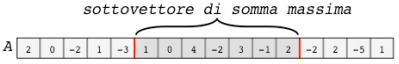
\includegraphics[width=0.5\linewidth]{images/es-sottolista.PNG}
    \caption{Sottolista che contiene valori positivi e negativi}
    \label{fig:es-sottolista}
\end{figure}
Un algoritmo diretto per il problema, basato sulla ricerca esaustiva, consiste nel considerare le somme di tutte le possibili sottoliste e prenderne il massimo:
\begin{lstlisting}[language=Python]
    def es(A):
        n=len(A)
        val=A[0]
        for i in range(n):
            for j in range(i,n):
                val=max(sum(A[i:j+1]),val)
        return val
\end{lstlisting}
L'algoritmo è molto inefficiente: la complessità è $O(n^3)$. Possiamo abbassare la complessità osservando che la somma di una sottolista \verb|[i...j]| è uguale alla somma della sottolista \verb|[i...j-1]| più \verb|lista[j]|.

\begin{lstlisting}[language=Python]
    def es(A):
        n=len(A)
        val=A[0]
        for i in range(n):
            s=0
            for j in range(i, n):
                s+=A[j]
                val=max(s, val)
        return val
\end{lstlisting}
L'algoritmo ha ora complessità $\Theta(n^2)$.
Possiamo fare di meglio? Le sottoliste possibili sono
\begin{equation*}
    \frac{n(n-1)}{2}+n=\frac{n(n + 1)}{2}= \Theta(n^2)    
\end{equation*}
Ma è realmente necessario esaminarle tutte per risolvere il problema? Proviamo ad applicare la tecnica del Divide et Impera. La prima cosa che viene in mente è di dividere a metà la lista, trovare il massimo in ciascuna delle due metà e poi calcolare il massimo delle somme delle sottoliste a cavallo delle due metà. Alla fine restituiamo il massimo dei tre massimi ottenuti.

Sicuramente l'algoritmo è corretto perché considera tutte le possibili sottoliste. Infatti, una sottolista o è contenuta interamente nella prima metà della lista o interamente nella seconda o è cavallo delle due metà.

Qual'è la sua complessità di questo algoritmo? La risposta dipende da come effettuiamo il calcolo delle somme delle sottoliste a cavallo. Se lo facciamo in modo diretto cioè, calcoliamo la somma della sottolista \verb|[i... j]| per ogni coppia di indici $i$ e $j$ con $i$ nella prima metà e $j$ nella seconda, questo richiede tempo $\Theta(n^2)$ (dato che il numero di sottoliste a cavallo è $\frac{n}{2}\frac{n}{2}= \Theta(n^2)$).

Ovviamente questo implica che la complessità $T(n)$ del nostro algoritmo Divide et Impera è determinata dalla relazione $T(n) = 2T\left(\frac{n}{2}\right) + \Theta(n^2)$ che risolta dà $T(n) = \Theta(n^2)$.

Possiamo migliorare il calcolo del massimo delle somme delle sottoliste a cavallo delle due metà? Osserviamo che ogni sottolista a cavallo è formato da un suffisso della prima metà della lista ed un prefisso della seconda metà della lista.

\begin{figure}[ht]
    \centering
    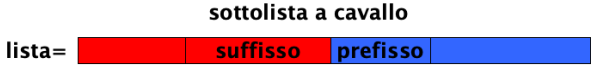
\includegraphics[width=0.5\linewidth]{images/es-sottolista-cavallo.PNG}
    \caption{Sottolista formata da prefisso e suffisso}
    \label{fig:es-sottolista-cavallo}
\end{figure}
La sottolista a cavallo di somma massima ha come valore il valore del suffisso di somma massima della prima metà della lista più il valore del prefisso di somma massima della seconda metà della lista.

\begin{lstlisting}[language=Python]
    def es(A):
        if len(A)==1: 
            return A[0]
        m=len(A)//2 
        rs=es(A[:m])
        rd=es(A[m:])
        pmax=x=A[m-1]
        for i in range(m-2,-1,-1):
            x+=A[i]
            pmax=max(pmax, x)
        smax=x=A[m]
        for i in range(m+1, len(A)):
            x+=A[i]
            smax=max(smax, x)
        return max(rs, rd, smax+pmax)
\end{lstlisting}
Il calcolo di \verb|A[:m]| e di \verb|A[m:]| costa $\Theta(n)$. Il calcolo del valore del suffisso massimo della prima metà di $A$ costa $\Theta(n)$. Il calcolo del valore del prefisso massimo della seconda metà di $A$ costa $\Theta(n)$. La ricorrenza che cattura la complessità $T(n)$ della funzione è
\begin{equation*}
    T(n) = 2T\left(\frac{n}{2}\right) + \Theta(n)
\end{equation*}
che risolta dà $\Theta(n\log n)$.

Si può fare di meglio? La risposta è si. Faremo ora vedere una migliore implementazione dell'algoritmo basato sul divide et impera che presenterà una complessità $\Theta(n)$. Nota che l'algoritmo $\Theta(n)$ sarà ottimo per il problema (il lower bound $\Omega(n)$ segue dalla banale osservazione che per risolvere il problema non si può fare a meno di scorrere tutti gli $n$ elementi della lista).
\begin{enumerate}
    \item Non possiamo permetterci di pagare $\Theta(n)$ in fase di invocazione della funzione sui due sottoproblemi (per la creazione di \verb|A[:m]| e \verb|A[m:]|) e per ovviare a questo problema indicheremo i sottoproblemi di $A$ con il loro punto di inizio $i$ ed il loro punto di fine $j$.
    \item Non possiamo permetterci di pagare $\Theta(n)$ in fase di combinazione delle risposte fornite dai due sottoproblemi. Per ovviare a questo problema faremo si che ogni sottoproblema restituisca ulteriore informazione che aiuti nella combinazione.
\end{enumerate}
Facciamo in modo che la procedura ricorsiva per $A$ con la soluzione $sol$ al problema restituisca anche altri tre valori (che semplificheranno poi il costo della combinazione): 
\begin{itemize}
    \item $tot$: la somma dei valori di $A$.
    \item $pm$: il valore massimo per i prefissi di $A$.
    \item $sm$: il valore massimo per i suffissi di $A$.
\end{itemize}
dai valori $solS$, $totS$, $pmS$ e $smS$ restituiti dal primo sottoproblema e dai valori $solD$, $totD$, $pmD$ e $smD$ restituiti dal secondo problema è possibile calcolare in $O(1)$:
\begin{itemize}
    \item \verb|sol = max{solS, solD, smS + pmD}|
    \item \verb|tot = totS + totD|
    \item \verb|pm = max{pmS, totS + pmD}|
    \item \verb|sm = max{smD, smS + totD}|
\end{itemize}

\begin{figure}[ht]
    \centering
    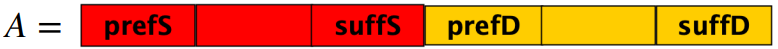
\includegraphics[width=0.5\linewidth]{images/es-sottolista-ric.PNG}
    \caption{Nuovi valori nella sottolista}
    \label{fig:es-sottolista-ric}
\end{figure}

\begin{lstlisting}[language=Python]
    def es(A, i, j):
        if i==j:
            return A[i], A[i], A[i], A[i]
        m=(i+j)//2
        sols, tots, pms, sms = es(A, i, m)
        sold, totd, pmd, smd = es(A, m+1, j)
        sol = max(sols, sold, sms + pmd)
        tot = tots + totd
        pm = max(pms, tots + pmd) 
        sm = max(smd, totd + sms)
        return sol, tot, pm, sm
\end{lstlisting}
La relazione di ricorrenza per il tempo di calcolo di questa implementazione è
\begin{equation*}
    T(n) = 2T\left(\frac{n}{2}\right) +\Theta(1)
\end{equation*}
che risolta dà $\Theta(n)$.

\subsection{Sottostringhe binarie}
\textit{Data una stringa binaria $S$ di $n$ bit progettare un algoritmo che calcoli il numero di sottostringhe di $S$ che cominciano con 0 terminano con 1. Progettare due algoritmi basati sulla tecnica del Divide et Impera, uno a complessità $\Theta(n\log n)$ e l'altro a complessità $\Theta(n)$.}

Ad esempio: per \verb|S ='0011'| restituisce 4 (infatti le sottostringhe sono \verb|001_|, \verb|0011|,\verb|_01__|,\verb|_011|). Per \verb|S = '0101'| restituisce 3 (infatti le sottostringhe sono \verb|01__|, \verb|0101|, \verb|__01|). Per \verb|S = '1100'| restituisce 0.

Divido la stringa in due sottostringhe di lunghezza circa $\frac{n}{2}$. Risolvo il problema in ciascuna delle due sottostringhe ricevendo come soluzione $ts$ e $td$. Restituisco il valore $ts+td+c$ dove $c$ è il numero di sottostringhe che iniziano nella sottostringa a destra e terminano nella sottostringa a sinistra. Per calcolare $c$ basta contare il numero $z$ degli zeri nella sottostringa di sinistra ed il numero $u$ degli uni nella sottostringa a destra (vale infatti $c=z*u$).

\begin{lstlisting}[language=Python]
    def es(S):
        if len(S)==1:
            return 0
        m = len(S)//2
        ts = es(S[:m])
        td = es(S[m:])
        return ts+td+S[:m].count('0')*S[m:].count('1')   
\end{lstlisting}
La relazione di ricorrenza per il tempo di calcolo di questa implementazione è:
\begin{equation*}
    T(n) = 2T\left(\frac{n}{2}\right) + \Theta(n)
\end{equation*}
che risolta dà $\Theta(n\log n)$.

Facciamo in modo che la funzione ricorsiva sulla stringa $S$ oltre a restituire il numero $t$ delle sottosequenze che cominciano con zero e finiscono con uno restituisca anche il numero $z$ dei suoi zeri e il numero $u$ dei suoi uni. Con queste informazioni da parte delle due chiamate ricorsive la funzione è in grado di calcolare in $\Theta(1)$ il numero di sottostringhe che cominciano nella sottostringa di sinistra e finiscono nella sottostringa di destra.

Sapendo infatti $zs$ (il numero di zeri della sottostringa di sinistra) e $ud$ (il numero di uni della sottostringa di destra) il numero di sottosequenze che iniziano alla sinistra del taglio e terminano alla destra del taglio sono $zs*ud$.

\begin{lstlisting}[language=Python]
    def es(S):
        if len(S)==1:
            if S[0]=='0': 
                return (1,0,0)
        else:
            return (0,1,0)
        m = len(S)//2
        zs, us, ts = es(S[:m]) 
        zd, ud, td = es(S[m:])
        return zs+zd, us+ud, ts+td+zs*ud
\end{lstlisting}
La relazione di ricorrenza per il tempo di calcolo di questa implementazione è ancora:
\begin{equation*}
    T(n) = 2T\left(\frac{n}{2}\right) + \Theta(n)
\end{equation*}
a causa del costo $\Theta(n)$ necessario per la creazione delle due istanze da invocare.
Il problema è facilmente risolvibile specificando le sottoliste da passare tramite indici di inizio e fine.

\begin{lstlisting}[language=Python]
    def es(S, i, j):
        if i==j:
            if S[i]=='0':
                return (1,0,0)
            else: 
                return (0,1,0)
        m = (i+j)//2
        zs, us, ts = es(S, i, m) 
        zd, ud, td = es(S, m+1, j)
        return zs+zd, us+ud, ts+td+zs*ud
\end{lstlisting}
La relazione di ricorrenza per il tempo di calcolo di questa implementazione è:
\begin{equation*}
    T(n) = 2T\left(\frac{n}{2}\right)+O(1)    
\end{equation*}
che risolta dà $\Theta(n)$.

